\section{Prime and extension fields}\label{sec:prime}

\subsection{Known-answer ladders over $\FF_p$}

Over prime fields the ledger tracks staged known-answer ladders
(\art{docs/ic/boundary_targets.json}, regime \texttt{prime}). On $j=0$
curves the staged driver recovers a 20-bit logarithm
($p=1{,}048{,}609$) in 56.8--64.9\,s of IC wall against 150--153\,ms of rho
on the identical public point, with split timers and three seeds. On the
generic $a=-3$ shape (P-256 and CryptoPro-B class), a Semaev-$\Sem4$
three-decomposition family with Cantor--Zassenhaus root finding yields one
relation per trial at $p=65{,}519$ with a 120-point base; at fixed base
size, median trials per relation grow from 2 to 28 to 379--506 at 16, 20
and 24 bits, about $16\times$ per four bits. The prime \texttt{vs\_rho}
row is \emph{not achieved} at any measured size.

\subsection{PDP oracle programme}

The point-decomposition (PDP) speed-up programme
(\art{research/pdp_oracle_speedup_20261011/}) measured the oracle in three
steps before root finding replaced it: a baseline (PS-0; $338$--$452$\,ns
per pair across five rungs, A/A spread $\le8.8\%$), a gate-count model of
the group-law form (PS-1; $7{,}410$--$14{,}608$ fused ternary-logic issues
against $70{,}695$--$190{,}275$ for the derived baseline, $9.5$--$13.0\times$),
and a scalar group-law kernel (PS-2; $29.8$--$40.8$\,ns per pair, per-pair
ratio to baseline $0.067$--$0.123$, 400 corpus root sets agreeing). A
split/hybrid solving-degree study then projected its closest relation phase
at $22.8\times$ strong rho (\art{research/pdp_split_dreg_20261011/}), with
an initial read-out defect preserved in the record.

\subsection{Kummer-tower factor bases}

Petit, Kosters and Messeng's base $V=\mu_{2^t}$ (the roots of
$x^{2^t}-1$) gives prime-field summation systems extra structure for an
algebraic solver. We ran it end to end in ecbench with the root-finding
oracles on five curves of 20--28 bits (896 runs, all verified, all replay
audits OK; \art{research/pkm_tower_ecbench_20261013/}). Index calculus
costs $34.0$, $41.9$, $29.4$, $96.6$ and $140.6\times$ rho-negation in $S$
(95\% intervals in Figure~\ref{fig:prime}), growing by $0.26\pm0.28$ bits of
$S_{IC}/S_\rho$ per bit of $r$, consistent with the $p^{1/6}$ the floors
predict. The tower base costs the same as a plain base of the same size to
within 1\% (ratios $0.999$--$1.012$): PKM's structure helps an algebraic
solver, not a table.

\subsection{Gaudry's $k=4$ index calculus over $\FF_{p^4}$}\label{sec:gaudry}

Over $\FF_{p^k}$ with a base of points whose abscissa lies in $\FF_p$, a
relation needs a $k$-decomposition solved by a Macaulay system. We made the
\texttt{gaudry\_quartic} solve generic in the number of unknowns and faster
(median whole solve $1.9$/$4.1$/$6.4\times$ at $d=4,5,6$, $37.4\to5.9$\,s
at $d=6$; the $\Sem5$ solve from about 30 minutes to 164--203\,s; every
count and solution identical). Then we built FGHR's $D_4$ variant
(\art{research/gaudry_quartic_d4_20261013/}): on a curve with rational
2-torsion $T$, the coordinate $Y=(x-x_0-c)/(x-x_0+c)$ satisfies
$Y(P+T)=-Y(P)$, so $\Sem5$ in $Y$ is invariant under the Weyl group $D_4$
(order 192). In the invariants $\sigma_k=e_k(Y^2)$, $\pi=\prod Y_i$, the
system has B\'ezout number 512 instead of 4{,}096, Macaulay degree 14
instead of 29, and a $13{,}412\times11{,}628$ matrix instead of
$41{,}780\times40{,}920$.

At $p=269$, the cost $C_4$ of one decomposition falls from
$1.21$--$1.23\cdot10^{12}$ to $2.54$--$2.55\cdot10^{10}$ $\FF_p$
multiplications, $47.5$--$48.4\times$; a solve takes 4.2--5.6\,s instead of
164--203\,s. Decompositions agree with an independent meet-in-the-middle
enumeration on 19 of 19 solved targets; one target in 20 is degenerate
(quotient dimension 517) and is discarded, adding about 5\% to the
relation phase. The $Y$-line base decomposes about $1/8$ as often (pooled
ratio $0.133$ over 8{,}000 targets; prediction $1/8\pm30\%$ held on one of
two curves), but each column covers $\{\pm P,\pm(P+T)\}$, halving the
unknowns.

Inserted into the repository's crossover model
(\art{research/notes/index-calculus/RESEARCH_RESIDUAL_WALKS.md} \S11.16), the measured $C_4$ and rate move
the $k=4$ crossover with rho from $2^{149.4}$--$2^{152.7}$ to
$2^{135.1}$--$2^{135.8}$ (cofactor $h=2$, forced by the 2-torsion), and
the asymptotic ratio past it from $0.34$--$0.63$ to $0.12$--$0.22$ of rho.
This is the one place in the programme where a crossover moves; it moves
in an \emph{extrapolated model} ($n^{1/4}$ relations, $n^{1/2}$ linear
algebra and rho) fed by a measured constant, so it is classed as
\cls{engineering}, not an advance. Extension fields of degree four are not
the fields deployed curves use.

\begin{figure}[t]
\centering
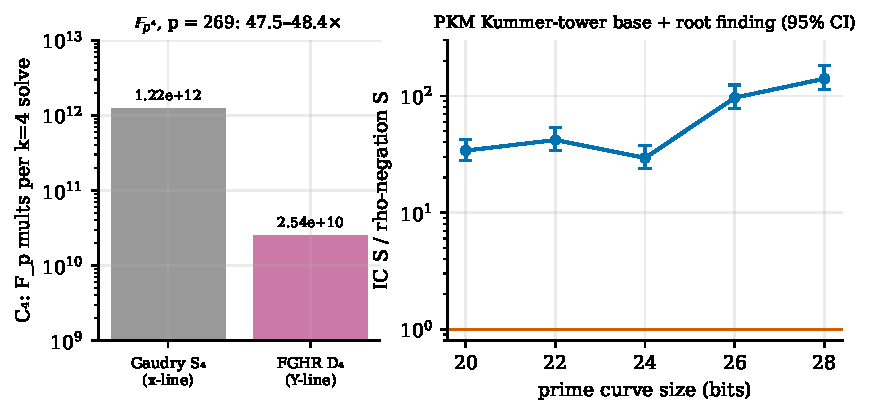
\includegraphics[width=\linewidth]{figures/fig-prime.pdf}
\caption[]{Left: cost $C_4$ of one $k=4$ decomposition over $\FF_{p^4}$,
$p=269$, Gaudry's $S_4$ system on the $x$-line against FGHR's $D_4$ system
on the $Y$-line (\art{research/gaudry_quartic_d4_20261013/}). Right:
index calculus with the PKM tower base and root finding over rho with
negation, eight one-target workloads $\times$ three rounds per size,
paired 95\% cluster-bootstrap intervals
(\art{research/pkm_tower_ecbench_20261013/}).}
\label{fig:prime}
\end{figure}

\subsection{Literature claims that did not survive}

The lit2026 programme (\art{research/lit2026_speedup_program/}) ran each
finding of a 2025--26 search as a measured change against an interleaved
baseline binary. Workstream W12 implemented the zero-minor
guess-and-determine attack (Mahalanobis, arXiv~2607.09814v2): it solved
48/48 planted targets on 16--26-bit curves, but its search phases scale
with slope $0.905$ $[0.769,1.021]$ in $\log_2 r$ and its cost over rho
grows from $260\times$ to $6{,}715\times$---exhaustive in $r$, as the
source's own table says. A second flagged ePrint (Hu, 2025/015) did not
specify an implementable algorithm and is recorded as blocked. On the
generic side, W11 cut BSGS from $16.75$ to $3.71$ multiplication
equivalents per visited point with paired steps (wall $1.15$--$1.67\times$),
which moves rho's and BSGS's constants, not index calculus.
